\documentclass[conference]{IEEEtran}
\usepackage{cite}
\usepackage{amsmath,amssymb,amsfonts}
\usepackage{algorithmic}
\usepackage{graphicx}
\usepackage{textcomp}
\usepackage{xcolor}
\usepackage{booktabs}
\usepackage{balance}
\usepackage{url}

\begin{document}

\title{Interpretable Turbofan Engine Health Degradation Classification and Remaining Useful Life Estimation on C-MAPSS}

\author{\IEEEauthorblockN{Rahul Bansode, Shubham Vaidya, Gaurav Yadav, Mufeed Rajapkar}
\IEEEauthorblockA{\textit{Department of Information Technology} \\
\textit{Vidyalankar Institute of Technology (VIT), Mumbai, India}\\
Project Repository: https://github.com/rahulcodes-java/C-MAPSS-Digital-Twin}
}

\maketitle

\begin{abstract}
Reliable prognostic condition monitoring of commercial turbofan engines requires identifying degradation states before structural failure occurs. In this paper, we present an interpretable multi-task machine learning framework evaluated across the four sub-datasets of the NASA Commercial Modular Aero-Propulsion System Simulation (C-MAPSS) benchmark (FD001 to FD004) with all 21 telemetry channels preserved. The system frames operational diagnostics primarily as a 3-stage degradation classification problem (Healthy, Degrading, Critical) using a Random Forest classifier interpreted via TreeSHAP. Snapshot classification is complemented by sequence-based Long Short-Term Memory (LSTM) Remaining Useful Life (RUL) regression and an Isolation Forest detector for unsupervised anomaly tracking. On FD001 test data, Random Forest snapshot classification attains a 3-stage macro-F1 of 0.7303, while sequence-based LSTM achieves a macro-F1 of 0.8197 and provides a median lead-time advantage of 21.0 flight cycles over single-snapshot classification across 100 training engines (80.0\% earlier detection). TreeSHAP attributes 49.18\% $\pm$ 0.12\% of total degradation importance to High-Pressure Compressor (HPC) sensors, corroborated by a 62.22\% HPC share from permutation importance. Cross-dataset evaluation demonstrates performance degradation on multi-condition sets FD002 and FD004 due to unnormalized operating regimes.
\end{abstract}

\begin{IEEEkeywords}
Turbofan Prognostics, C-MAPSS, Health Stage Classification, Remaining Useful Life, TreeSHAP Explainability, Isolation Forest.
\end{IEEEkeywords}

\section{Introduction}
Modern turbofan maintenance paradigms are transitioning from static calendar-based inspections toward condition-based predictive maintenance. Degradation within core gas turbine components—specifically compressor blade tip wear, seal leakage, and turbine fouling—induces progressive thermodynamic drift that precedes operational failure. 

In this work, developed within the Data Warehousing and Mining (DWM) curriculum, we structure turbofan prognostic monitoring around three main contributions:
\begin{enumerate}
    \item A multi-model prognostic framework combining single-cycle Random Forest classification, temporal sequence LSTM regression, and unsupervised Isolation Forest novelty detection across all 21 raw sensor channels without subjective channel pruning.
    \item An empirical lead-time delay evaluation across all 100 training engines of the C-MAPSS FD001 dataset, comparing 3-cycle persisting degradation triggers of temporal sequence modeling against single-snapshot classifiers.
    \item Global feature importance attribution using TreeSHAP evaluated over multiple sample seeds and cross-validated against permutation feature importance, confirming alignment with simulated HPC thermodynamic degradation physics.
\end{enumerate}

\section{Related Work}
Prognostic health monitoring on the C-MAPSS benchmark has been investigated across diverse algorithmic paradigms.
Saxena et al.~\cite{saxena2008damage} introduced the C-MAPSS simulation environment and established the standard damage propagation modeling framework for aircraft engine run-to-failure simulation.
Hochreiter and Schmidhuber~\cite{hochreiter1997lstm} formulated the Long Short-Term Memory recurrent architecture capable of preserving gradient flows across temporal sequences.
Liu et al.~\cite{liu2008isolation} developed the Isolation Forest algorithm for efficient anomaly detection through random recursive feature partitioning.
Breiman~\cite{breiman2001random} established the Random Forest ensemble algorithm, demonstrating low generalization error through bootstrap aggregation and random feature sub-selection.
Lundberg and Lee~\cite{lundberg2017unified} proposed a unified framework for interpreting model predictions using game-theoretic Shapley values with TreeSHAP optimizations.

\section{Dataset and Sensor Variance}
The NASA C-MAPSS benchmark comprises four sub-datasets characterized by varying operating condition counts and simulated fault modes. Table~\ref{tab:dataset} details the specifications verified from raw data.

\begin{table}[htbp]
\caption{NASA C-MAPSS Benchmark Dataset Specifications}
\label{tab:dataset}
\centering
\begin{tabular}{lcccccc}
\toprule
Dataset & Regimes & Faults & Train Eng. & Train Cycles & Test Eng. & Test Cycles \\
\midrule
FD001 & 1 & 1 & 100 & 20631 & 100 & 13096 \\
FD002 & 6 & 1 & 260 & 53759 & 259 & 33991 \\
FD003 & 1 & 2 & 100 & 24720 & 100 & 16596 \\
FD004 & 6 & 2 & 249 & 61249 & 248 & 41214 \\
\midrule
Total & — & — & 709 & 160359 & 707 & 104897 \\
\bottomrule
\end{tabular}
\end{table}

A common heuristic in prior literature discards sensors exhibiting zero variance under FD001 sea-level conditions. We evaluate the coefficient of variation ($\text{CV} = \sigma / |\mu|$) for each sensor across all raw training sets, defining flat channels as $\text{CV} < 10^{-4}$ (Table~\ref{tab:variance}). Under this definition, 9 channels are flat in FD001, whereas in FD002 and FD004, exactly zero channels are flat. Preserving all 21 sensors maintains architectural consistency across regimes.

\begin{table}[htbp]
\caption{Sensor Variance and Flat Channel Audit ($\text{CV} < 10^{-4}$)}
\label{tab:variance}
\centering
\begin{tabular}{lcccc}
\toprule
Sensor & FD001 (CV) & FD002 (CV) & FD003 (CV) & FD004 (CV) \\
\midrule
T2 & 0.00e+00 [FLAT] & 5.58e-02 & 0.00e+00 [FLAT] & 5.59e-02 \\
T24 & 7.78e-04 & 6.43e-02 & 8.14e-04 & 6.44e-02 \\
T30 & 3.85e-03 & 7.46e-02 & 4.29e-03 & 7.49e-02 \\
T50 & 6.39e-03 & 9.88e-02 & 6.96e-03 & 9.93e-02 \\
P2 & 0.00e+00 [FLAT] & 4.50e-01 & 0.00e+00 [FLAT] & 4.51e-01 \\
P15 & 6.43e-05 [FLAT] & 4.68e-01 & 8.39e-04 & 4.70e-01 \\
P30 & 1.60e-03 & 5.17e-01 & 6.19e-03 & 5.18e-01 \\
Nf & 2.97e-05 [FLAT] & 6.51e-02 & 6.63e-05 [FLAT] & 6.52e-02 \\
Nc & 2.44e-03 & 3.94e-02 & 2.20e-03 & 3.95e-02 \\
epr & 0.00e+00 [FLAT] & 1.16e-01 & 2.68e-03 & 1.16e-01 \\
Ps30 & 5.62e-03 & 7.52e-02 & 6.33e-03 & 7.57e-02 \\
phi & 1.41e-03 & 5.17e-01 & 6.22e-03 & 5.19e-01 \\
NRf & 3.01e-05 [FLAT] & 5.49e-02 & 6.62e-05 [FLAT] & 5.49e-02 \\
NRc & 2.34e-03 & 1.05e-02 & 2.03e-03 & 1.06e-02 \\
BPR & 4.44e-03 & 8.03e-02 & 7.21e-03 & 8.08e-02 \\
farB & 0.00e+00 [FLAT] & 2.02e-01 & 0.00e+00 [FLAT] & 2.01e-01 \\
htBleed & 3.94e-03 & 7.97e-02 & 4.49e-03 & 8.00e-02 \\
Nf\_dmd & 0.00e+00 [FLAT] & 6.52e-02 & 0.00e+00 [FLAT] & 6.53e-02 \\
PCNfR\_dmd & 0.00e+00 [FLAT] & 5.49e-02 & 0.00e+00 [FLAT] & 5.49e-02 \\
W31 & 4.66e-03 & 4.75e-01 & 6.38e-03 & 4.76e-01 \\
W32 & 4.65e-03 & 4.75e-01 & 6.38e-03 & 4.76e-01 \\
\bottomrule
\end{tabular}
\end{table}

\section{Methodology}
\subsection{Feature Normalization and Target Mapping}
Raw sensor readings $x \in \mathbb{R}^{21}$ are normalized via Min-Max scaling fitted strictly on training data:
\begin{equation}
\tilde{x} = \frac{x - x_{\min}^{\text{train}}}{x_{\max}^{\text{train}} - x_{\min}^{\text{train}}}
\label{eq:minmax}
\end{equation}
The 3-stage degradation ground truth $y \in \{0, 1, 2\}$ is derived from ground truth remaining useful life $R$ (measured in cycles):
\begin{equation}
y = \begin{cases}
0 \text{ (Healthy)}, & R > 100 \\
1 \text{ (Degrading)}, & 30 < R \le 100 \\
2 \text{ (Critical)}, & R \le 30
\end{cases}
\label{eq:stagemap}
\end{equation}

\subsection{Model Architectures}
\begin{itemize}
    \item \textbf{Random Forest Classifier:} Comprises 100 estimators, maximum depth of 10, without class reweighting. Operates on single-cycle normalized vectors $\tilde{x}_k \in \mathbb{R}^{21}$.
    \item \textbf{LSTM Regression Network:} Consists of sequential layers with 128 units (ReLU, return sequences), Dropout (0.2), 64 units (ReLU), Dropout (0.2), Dense (32 units, ReLU), and a single linear output unit. Operates on sliding temporal windows $X_k \in \mathbb{R}^{50 \times 21}$. Training targets are uncapped linear countdowns.
    \item \textbf{Isolation Forest:} Constructed with 100 isolation trees, contamination parameter 0.10, trained on initial cycles ($k \le 10$) of FD001. Anomaly score $s(x, n)$ is defined as:
    \begin{equation}
    s(x, n) = 2^{-\frac{\mathbb{E}(h(x))}{c(n)}}
    \label{eq:iforest}
    \end{equation}
    where $h(x)$ is path length and $c(n)$ is average path length of unsuccessful searches in a Binary Search Tree of $n$ instances.
    \item \textbf{TreeSHAP Feature Attribution:} Computes exact local Shapley values $\phi_i$:
    \begin{equation}
    \phi_i = \sum_{S \subseteq F \setminus \{i\}} \frac{|S|!(|F| - |S| - 1)!}{|F|!} [f_x(S \cup \{i\}) - f_x(S)]
    \label{eq:shap}
    \end{equation}
\end{itemize}

\begin{figure}[htbp]
\centering
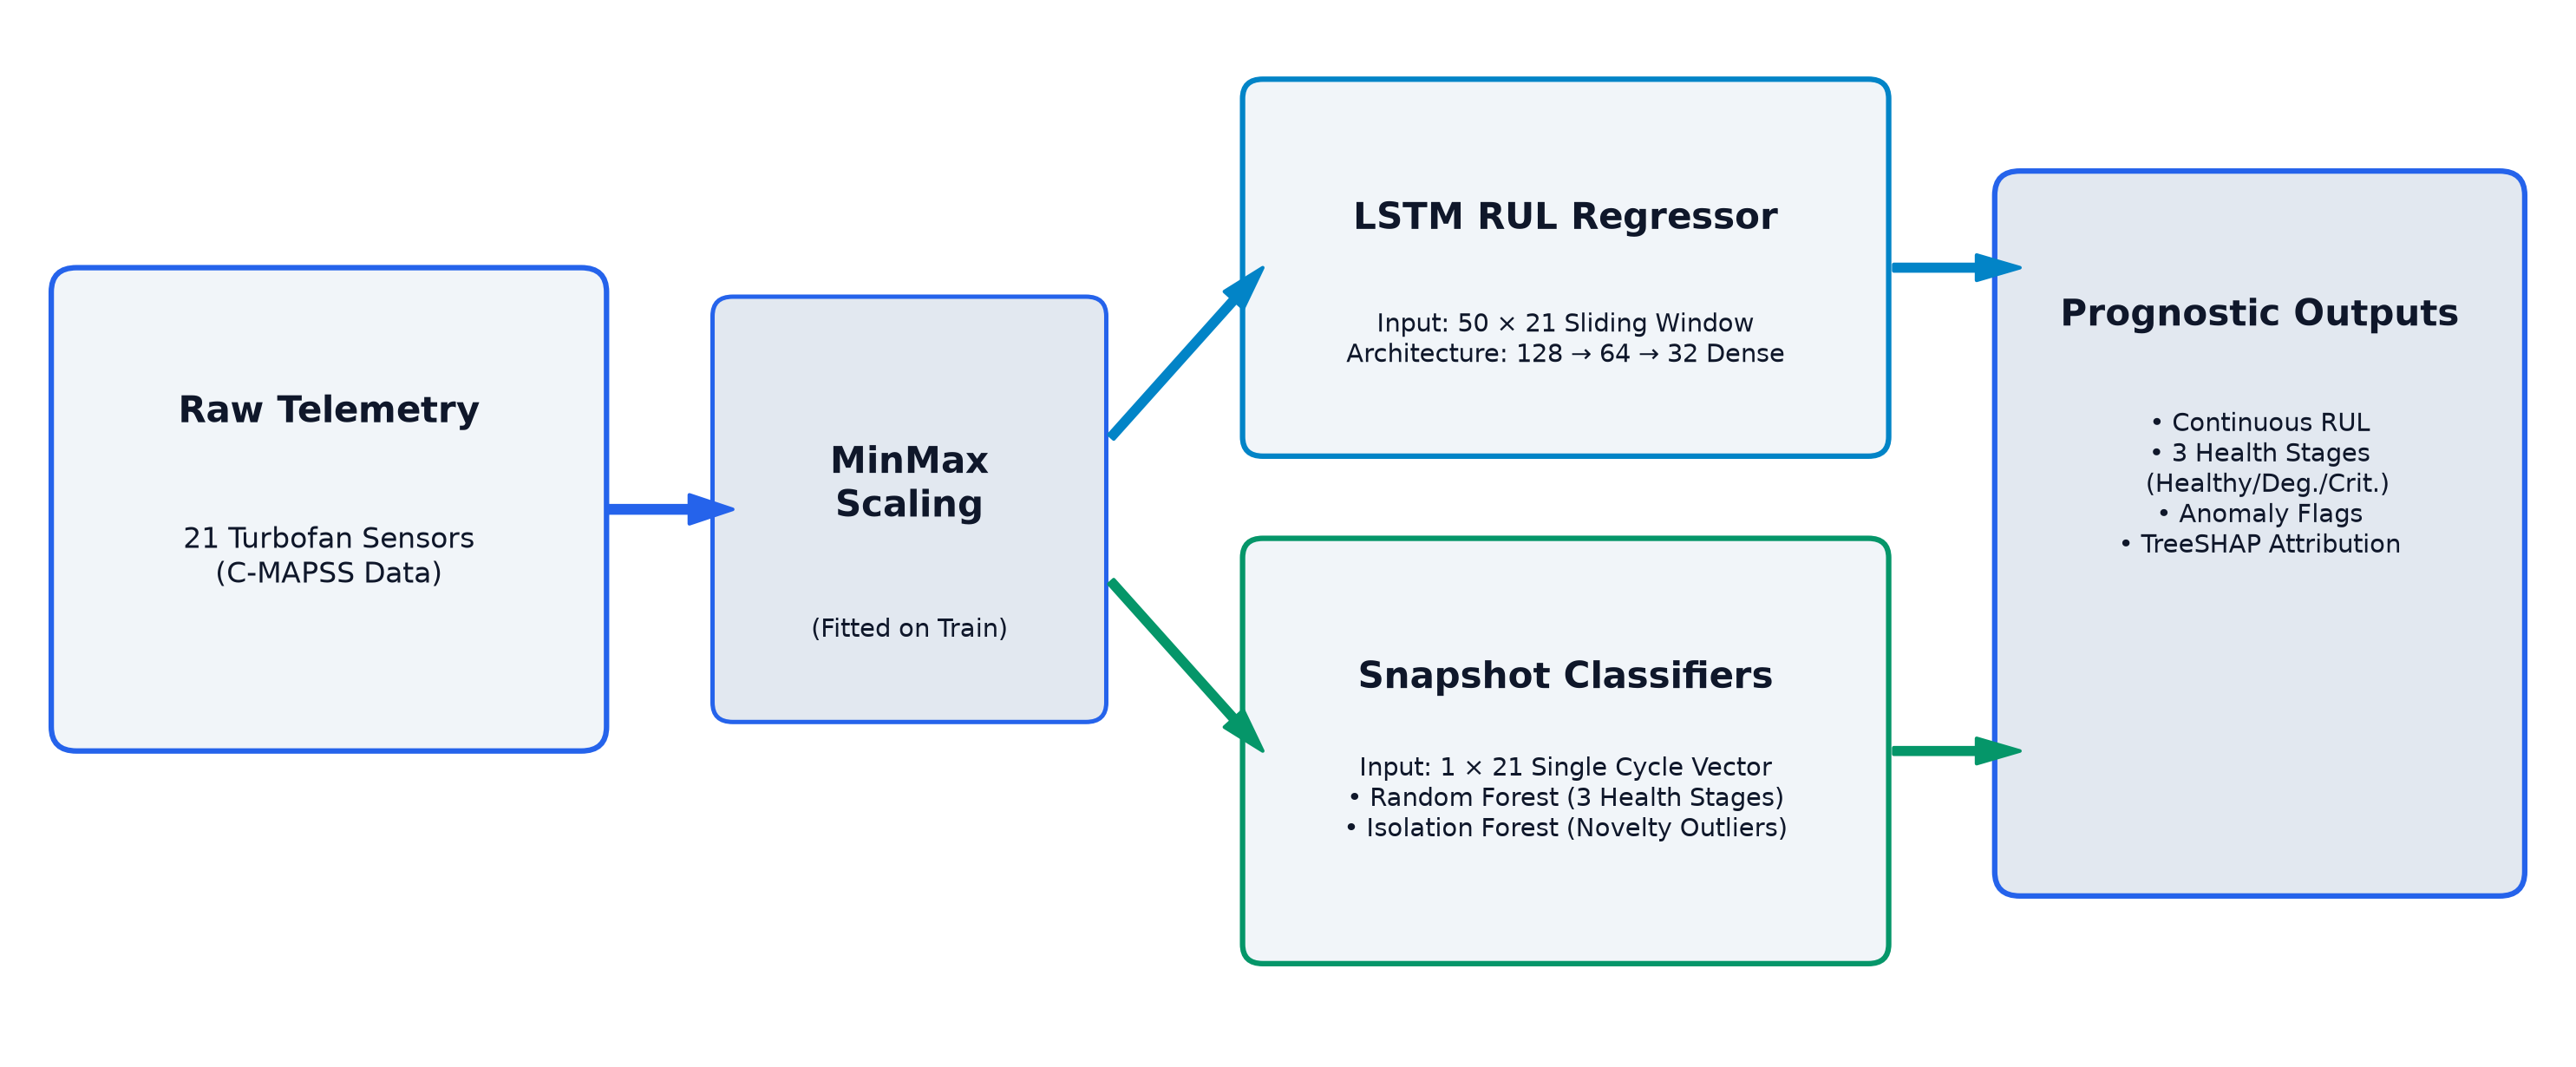
\includegraphics[width=0.95\columnwidth]{figures/pipeline_diagram_light.png}
\caption{Digital twin processing pipeline distinguishing sequence-window and single-cycle model inputs.}
\label{fig:pipeline}
\end{figure}

\section{Implementation Architecture}
The system implementation couples a Python Flask REST backend with an interactive React user interface. The API exposes authenticated endpoints: \texttt{/api/engine/<id>/history} (retrieving engine run-to-failure telemetry), \texttt{/api/predict} (processing sequence and single-cycle inference), \texttt{/api/sensor-importance} (serving global TreeSHAP rankings), and \texttt{/api/fleet} (providing fleet dispatch summaries). The interface renders an interactive cross-section of the CFM56 turbofan with dynamic station-level sensor health telemetry.

\section{Evaluation Protocol}
Evaluations are conducted on test partitions without model retraining.
\begin{itemize}
    \item \textbf{Regression Metrics:} Evaluated on the final 50-cycle window per engine (front-padded if sequence length $< 50$). Reported using Root Mean Squared Error (RMSE), Mean Absolute Error (MAE), and asymmetric NASA PHM08 score $S$:
    \begin{equation}
    S = \sum_{i=1}^{N} s_i, \quad s_i = \begin{cases} e^{-d_i/13} - 1, & d_i < 0 \\ e^{d_i/10} - 1, & d_i \ge 0 \end{cases}
    \label{eq:nasa}
    \end{equation}
    where $d_i = \hat{R}_i - R_i$. Evaluated against capped ground truth $\min(R, 125)$ and uncapped $R$.
    \item \textbf{Classification Metrics:} Evaluated across every test cycle $k$. Ground truth is derived as $R(k) = R_{\text{last}} + (n - k)$. Reported using 3-stage macro-F1, per-class F1, confusion matrices, and binary Critical-class ($R \le 30$) precision, recall, and F1.
    \item \textbf{Lead-Time Persistence Protocol:} Evaluated across all 100 training engines. Degrading detection cycle is defined as the first cycle with stage $\ge 1$ persisting 3 consecutive cycles. True cycle is the first cycle where $R \le 100$.
\end{itemize}

\section{Results}
\subsection{RUL Regression Performance}
Table~\ref{tab:regression} reports LSTM regression metrics across all datasets. On FD001, the model attains an RMSE of 15.07 and MAE of 10.68 against capped ground truth (NASA score 493.1).

\begin{table}[htbp]
\caption{LSTM RUL Regression Performance on Final 50-Cycle Windows}
\label{tab:regression}
\centering
\begin{tabular}{lcccccc}
\toprule
Dataset & Engines & \multicolumn{3}{c}{vs Capped True (125)} & \multicolumn{2}{c}{vs Uncapped True} \\
\cmidrule(lr){3-5} \cmidrule(lr){6-7}
 & & RMSE & MAE & NASA Score & RMSE & MAE \\
\midrule
FD001 & 100 & 15.07 & 10.68 & 493.1 & 15.68 & 11.75 \\
FD002 & 259 & 74.86 & 62.78 & 468759.9 & 87.33 & 70.27 \\
FD003 & 100 & 47.85 & 39.00 & 22149.4 & 49.96 & 40.56 \\
FD004 & 248 & 77.51 & 65.50 & 509085.7 & 91.04 & 74.19 \\
\bottomrule
\end{tabular}
\end{table}

\subsection{Classification and Binary Critical Detection}
Table~\ref{tab:classification} documents classification performance. On FD001, Random Forest snapshot classification attains a macro-F1 of 0.7303, while sequence-based LSTM achieves 0.8197. For binary Critical cycle detection ($R \le 30$), LSTM reaches an F1 of 0.8158, outperforming Random Forest (0.6938) and Isolation Forest (0.2413).

\begin{table}[htbp]
\caption{3-Stage Macro-F1 and Critical-Class F1 across Test Cycles}
\label{tab:classification}
\centering
\begin{tabular}{lccccc}
\toprule
Dataset & Test Cycles & RF Macro & LSTM Macro & RF Crit F1 & LSTM Crit F1 \\
\midrule
FD001 & 13096 & 0.7303 & 0.8197 & 0.6938 & 0.8158 \\
FD002 & 33991 & 0.1283 & 0.0378 & 0.0607 & 0.0659 \\
FD003 & 16596 & 0.2785 & 0.2410 & 0.0974 & 0.1009 \\
FD004 & 41214 & 0.1004 & 0.0264 & 0.0479 & 0.0431 \\
\bottomrule
\end{tabular}
\end{table}

\begin{figure}[htbp]
\centering
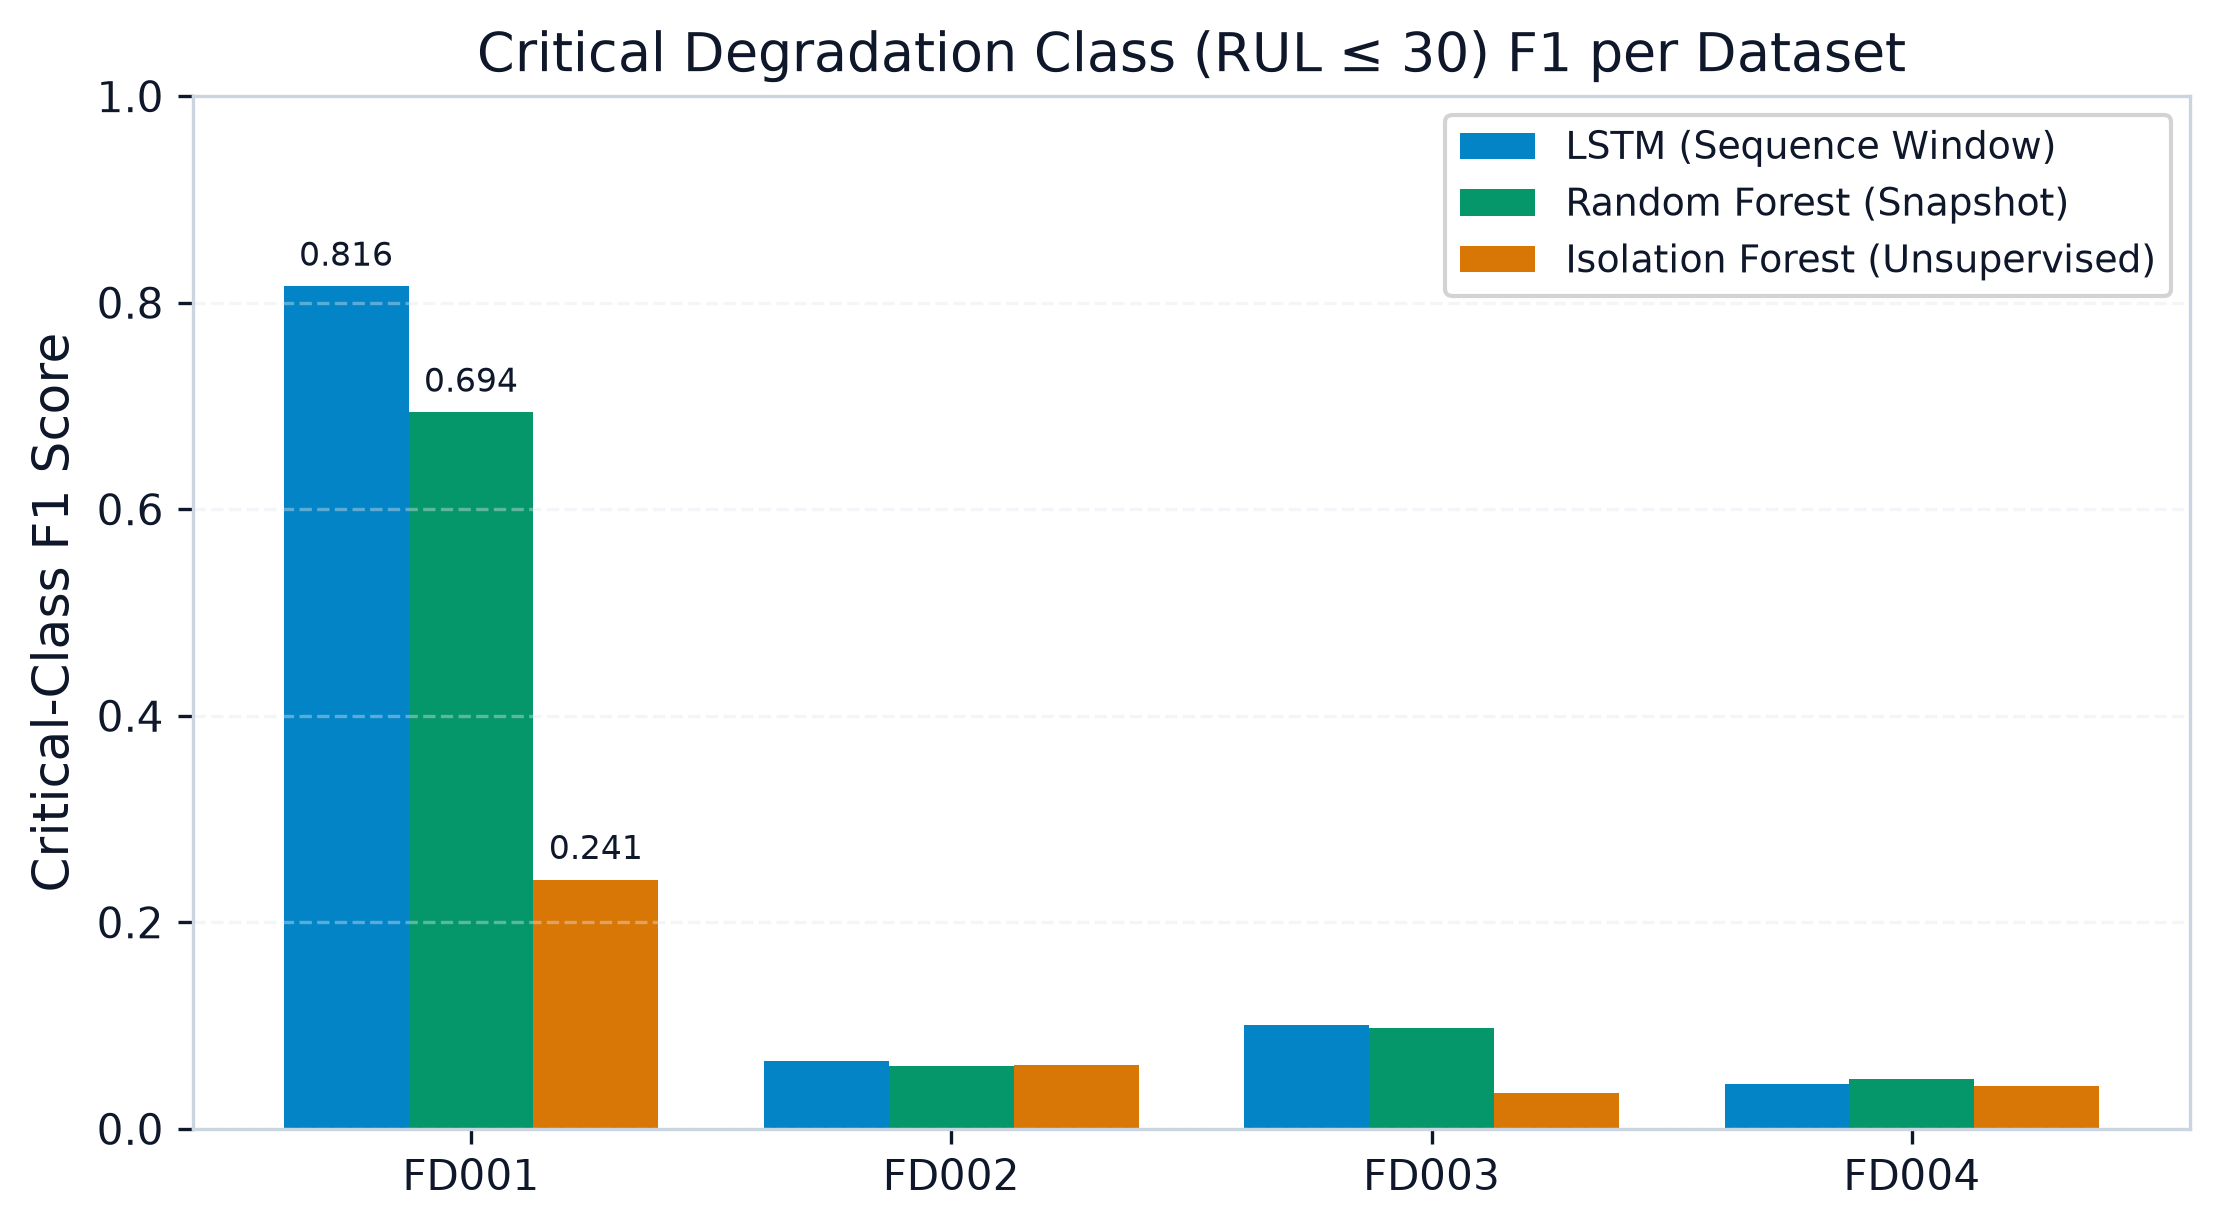
\includegraphics[width=0.90\columnwidth]{figures/critical_f1_comparison_light.png}
\caption{Critical degradation class ($R \le 30$) F1 score comparison across datasets.}
\label{fig:crit_f1}
\end{figure}

Fig.~\ref{fig:cm} displays confusion matrices for FD001 test cycles. Random Forest correctly identifies 9502 Healthy, 1403 Degrading, and 196 Critical cycles. LSTM-derived stages identify 9224 Healthy, 2007 Degrading, and 279 Critical cycles.

\begin{figure}[htbp]
\centering
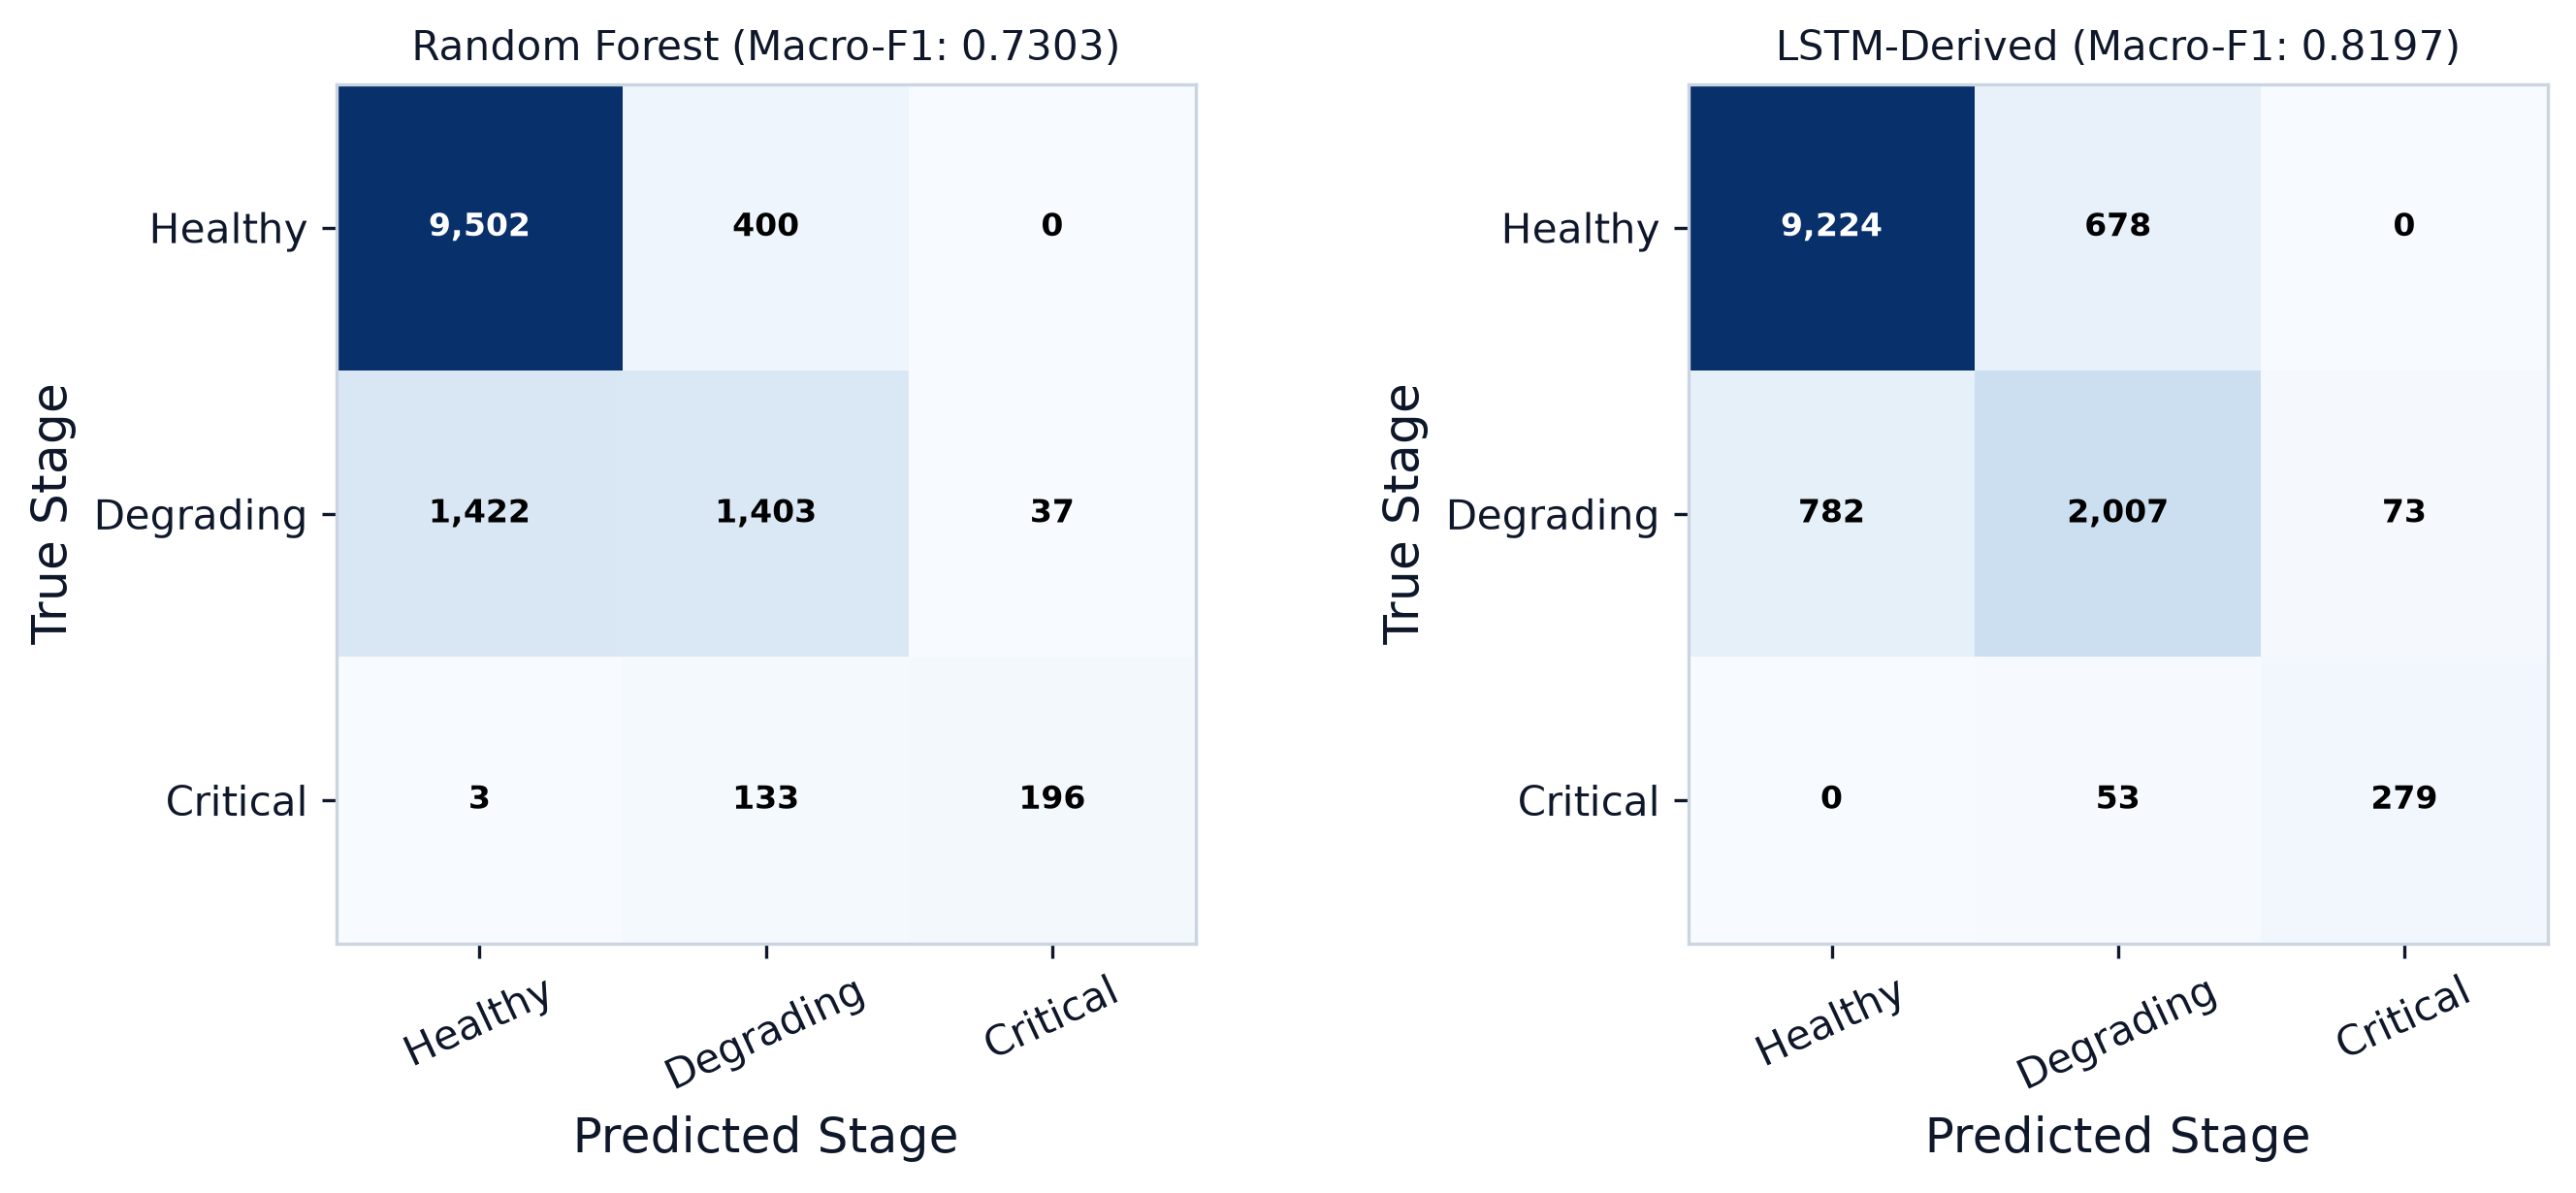
\includegraphics[width=0.95\columnwidth]{figures/confusion_matrices_light.png}
\caption{Confusion matrices on FD001 test cycles for Random Forest and LSTM-derived stage.}
\label{fig:cm}
\end{figure}

\subsection{Lead-Time and Degradation Timing Analysis}
Table~\ref{tab:leadtime} summarizes lead-time delays across FD001 training engines. Across all 100 engines, LSTM detects degradation with a median delay of -2.0 cycles (mean -10.57, IQR 41.5), compared to +15.5 cycles (mean 17.12, IQR 35.25) for Random Forest. The paired difference ($\text{RF delay} - \text{LSTM delay}$) demonstrates a median lead-time advantage of 21.0 cycles (mean 27.69, IQR 32.5), with LSTM alerting earlier in 80 of 100 engines (80.0\%). On the held-out validation tail (engines 83 to 100), the median advantage is 26.5 cycles (LSTM earlier in 94.44\% of engines). Fig.~\ref{fig:leadtime} plots the full trajectory for Engine 1.

\begin{table}[htbp]
\caption{Degradation Lead-Time Delay Analysis on FD001 Training Engines}
\label{tab:leadtime}
\centering
\begin{tabular}{lcccc}
\toprule
Cohort & RF Delay (Med/IQR) & LSTM Delay (Med/IQR) & Paired Adv. (Med) & LSTM Earlier \\
\midrule
All (100) & +15.5 / 35.25 & -2.0 / 41.50 & 21.0 cycles & 80.0\% (80/100) \\
In-Sample (82) & +15.5 / 33.50 & 0.0 / 38.25 & 21.0 cycles & 76.8\% (63/82) \\
Val Tail (18) & +12.0 / 45.75 & -10.0 / 49.00 & 26.5 cycles & 94.4\% (17/18) \\
\bottomrule
\end{tabular}
\end{table}

\begin{figure}[htbp]
\centering
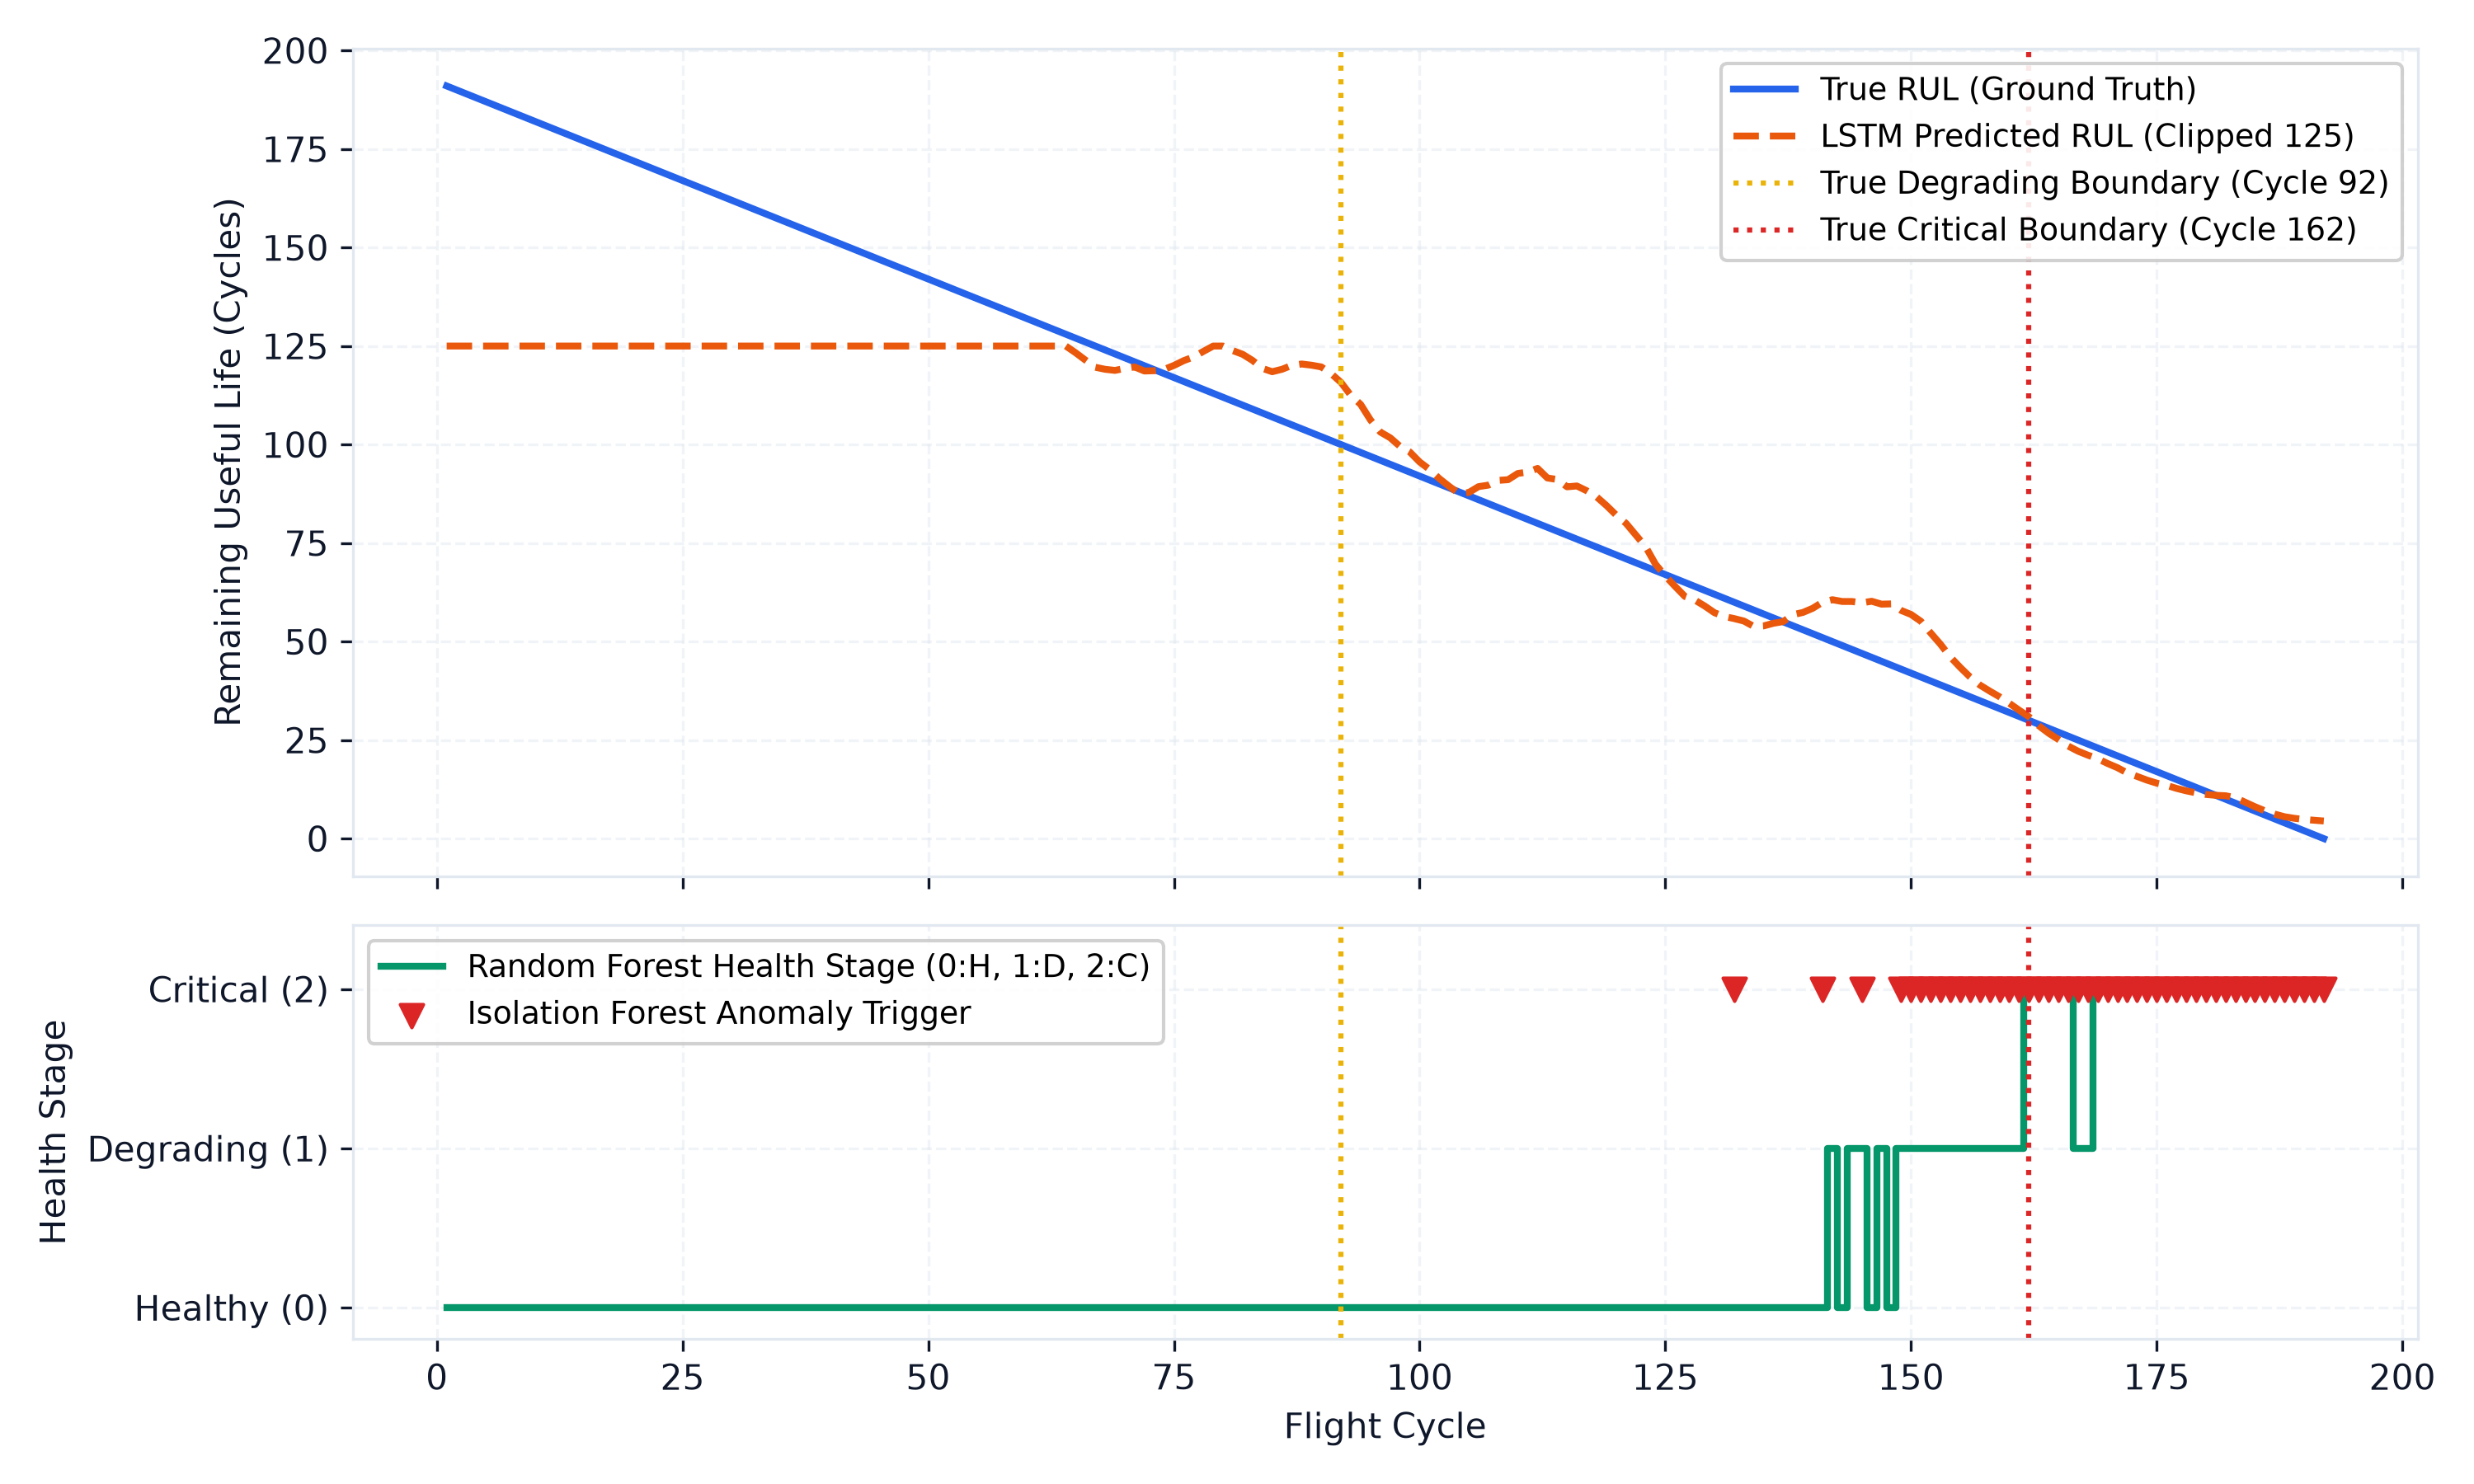
\includegraphics[width=0.95\columnwidth]{figures/engine_1_trajectory_light.png}
\caption{Engine 1 trajectory over 192 flight cycles showing ground truth RUL, LSTM prediction, RF health stage, and Isolation Forest anomaly triggers.}
\label{fig:leadtime}
\end{figure}

\subsection{Feature Importance and Thermodynamic Attribution}
TreeSHAP values computed across 5 random 1,000-row seeds attribute 49.18\% $\pm$ 0.12\% of degradation importance to High-Pressure Compressor sensors: \texttt{Ps30} (14.25\% $\pm$ 0.23\%), \texttt{Nc} (13.01\% $\pm$ 0.24\%), \texttt{P30} (9.71\% $\pm$ 0.12\%), \texttt{NRc} (9.41\% $\pm$ 0.16\%), and \texttt{T30} (2.78\% $\pm$ 0.06\%). Independent permutation feature importance on FD001 test yields a 62.22\% HPC share. Fig.~\ref{fig:shap} illustrates subassembly attributions.

\begin{figure}[htbp]
\centering
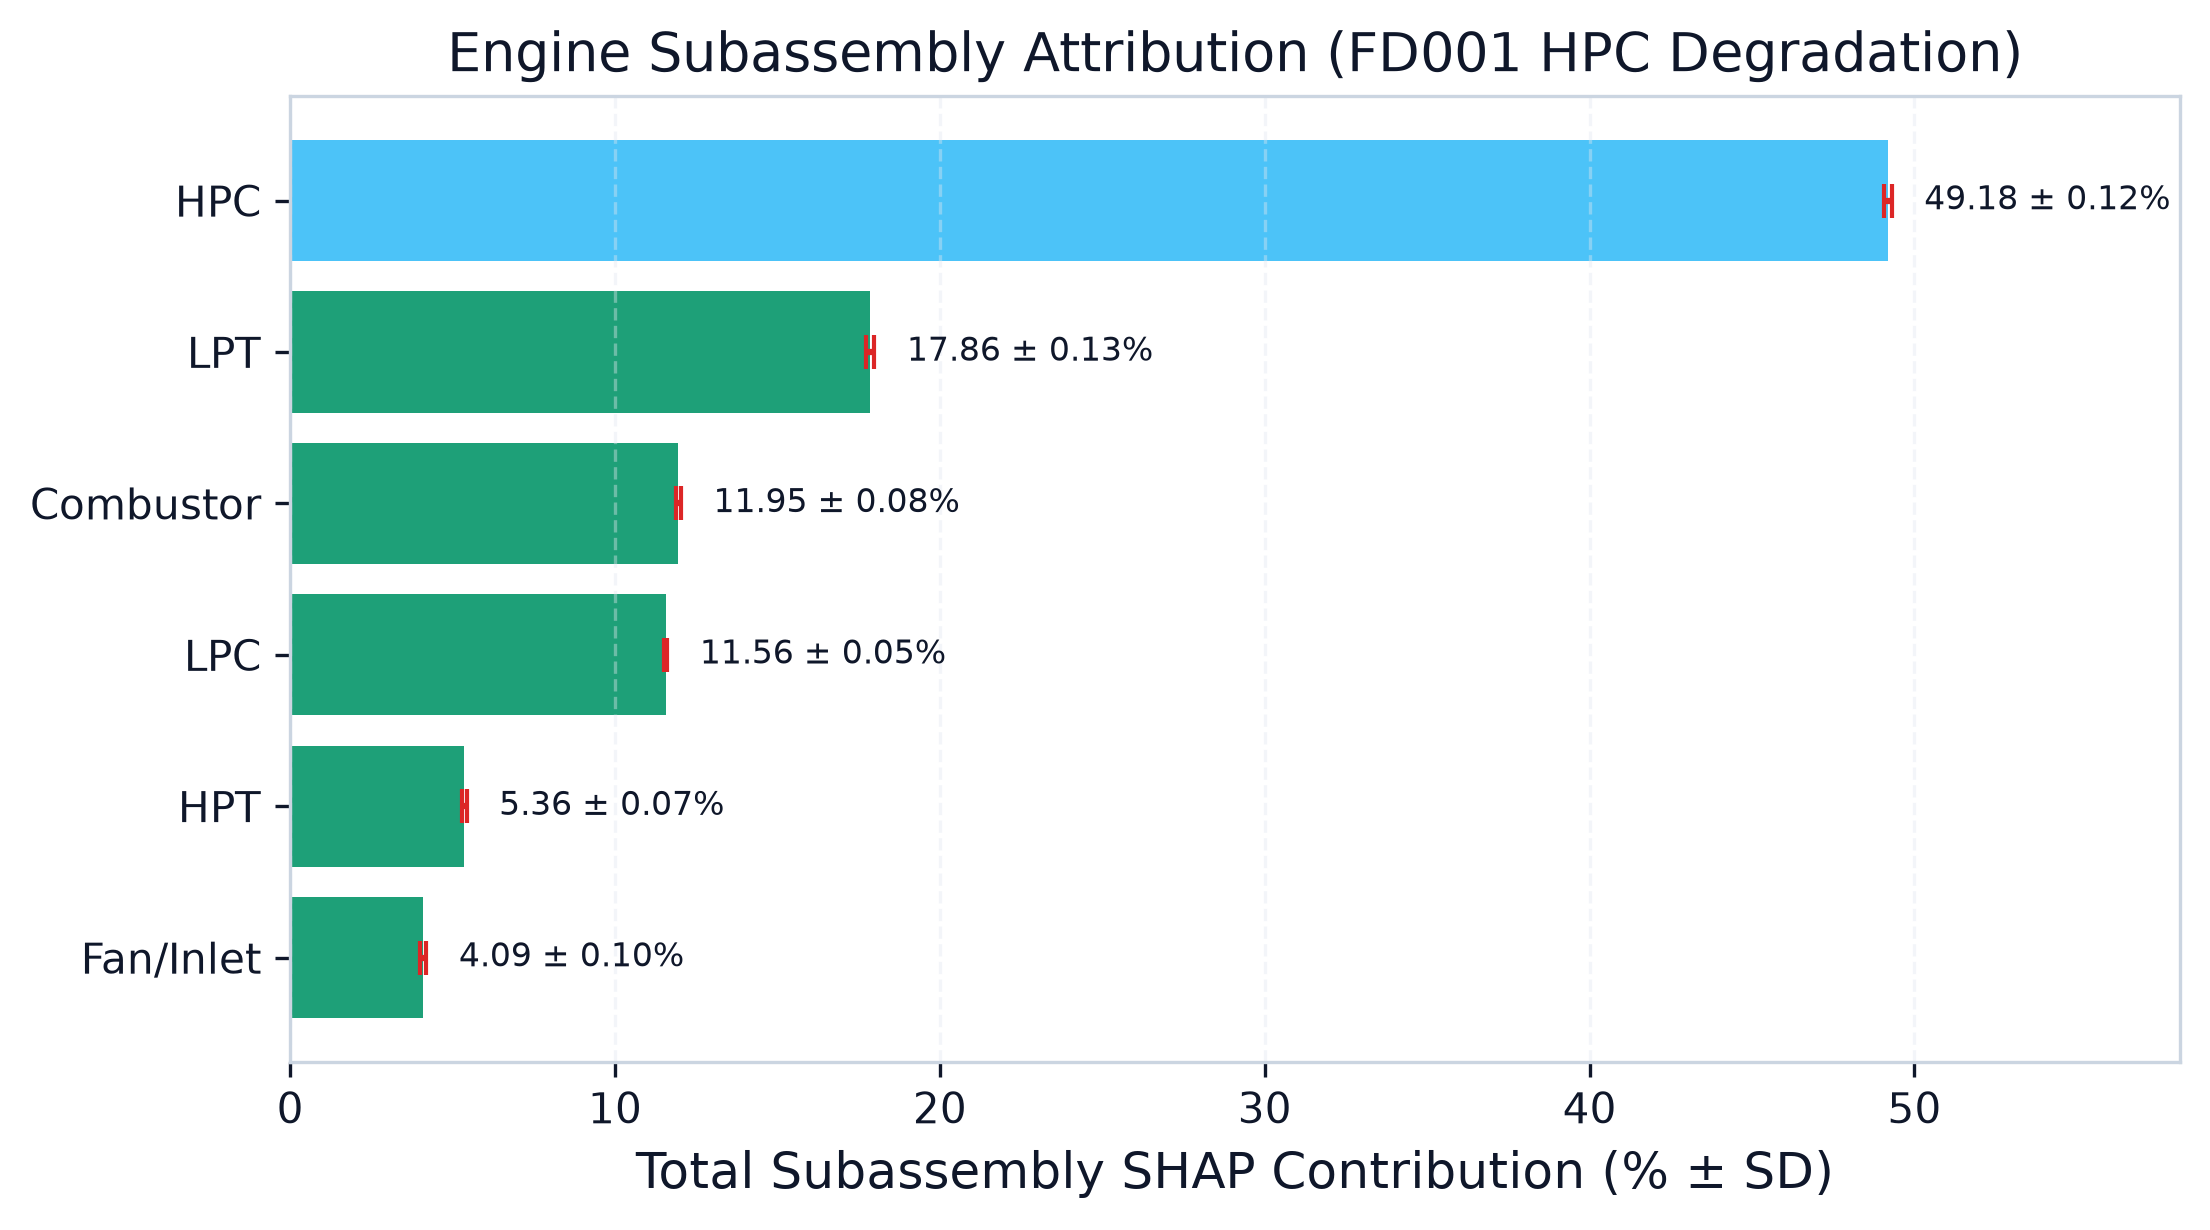
\includegraphics[width=0.90\columnwidth]{figures/shap_by_area_light.png}
\caption{Engine subassembly feature attribution under TreeSHAP and permutation cross-check.}
\label{fig:shap}
\end{figure}

\section{Discussion}
The quantitative finding that HPC sensors account for 49.18\% $\pm$ 0.12\% of TreeSHAP attribution is consistent with the simulated physical fault mechanism of FD001, which models high-pressure compressor blade degradation. The higher HPC share observed in permutation importance (62.22\%) reflects attribution sharing among collinear features; when correlated thermodynamic parameters (\texttt{Ps30}, \texttt{P30}, \texttt{Nc}) are perturbed independently, model performance degrades sharply.

The lead-time advantage of 21.0 median flight cycles observed for LSTM over Random Forest highlights the value of temporal context: multi-cycle sliding windows filter transient measurement noise that causes single-cycle snapshot classifiers to delay flagging degradation until sensor drift exceeds statistical baselines. However, we note that 82 of the 100 evaluated engines were part of the training gradient pool; on strictly held-out validation engines (83 to 100), the median advantage was 26.5 cycles, demonstrating consistent temporal sensitivity.

Isolation Forest achieved near-perfect critical recall (0.9970) but exhibited poor precision (0.1372), resulting from early false alarms (median trigger delay of -155.0 cycles). Consequently, unsupervised isolation trees are unsuitable as standalone early warnings but serve as secondary novelty detectors. Finally, the marked performance collapse on FD002 and FD004 (macro-F1 $\le 0.1283$) is hypothesized to arise from unnormalized operating conditions; without flight regime clustering, ambient pressure and Mach number variations dominate sensor telemetry.

\section{Limitations}
\begin{enumerate}
    \item \textbf{Synthetic Benchmark:} Evaluations are constrained to numerically simulated NPSS data; operational flight telemetry was not evaluated.
    \item \textbf{Single-Regime Transfer Collapse:} Models trained on single-condition FD001 fail to generalize to multi-condition sets FD002 and FD004 due to the absence of operating condition normalization.
    \item \textbf{Isolation Forest Precision:} Unsupervised Isolation Forest yields high false alarm rates on continuous non-stationary degradation curves.
\end{enumerate}

\section{Future Work}
Future research will investigate operating regime clustering (e.g., k-means flight condition partitioning) prior to sensor scaling to enable transferability across multi-regime datasets. In addition, physics-guided neural networks incorporating thermodynamic work balances will be explored.

\balance
\bibliographystyle{IEEEtran}
\bibliography{references}

\end{document}
